\section{Data and methods}
\label{sec:methods}

Two recognizers transcribe each conversation: Parakeet, fine-tuned on the tapes, and Whisper, unchanged. A merge keeps Parakeet's words and attaches Whisper's reading at every disagreement. A language model corrects the merged text against the archive and returns edits. A voiceprint classifier labels the speakers (Figure~\ref{fig:pipeline}). The release keeps every layer.

\begin{figure}[t]
  \centering
  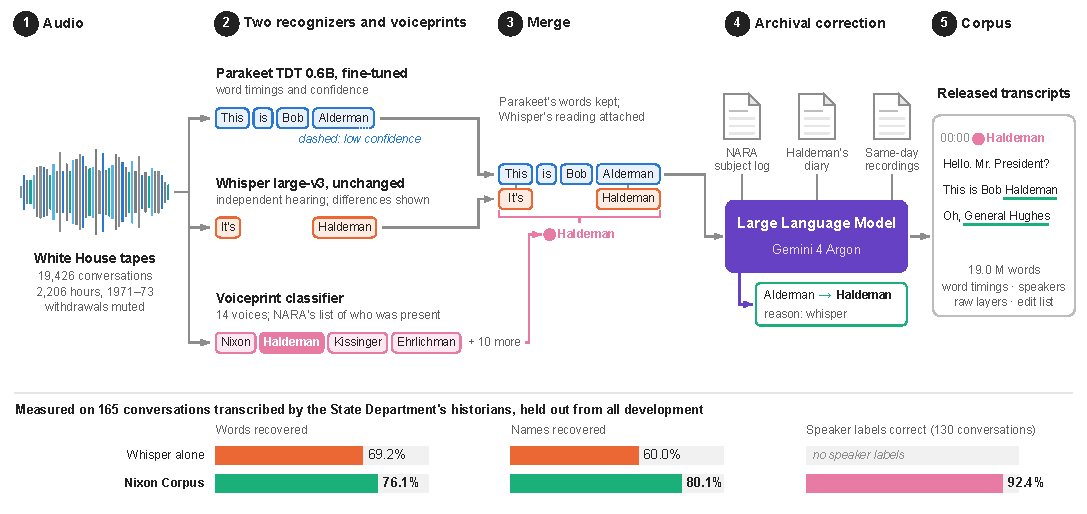
\includegraphics[width=\linewidth]{figures/fig1_pipeline.pdf}
  \caption{The pipeline, followed through one moment of the corpus: Haldeman giving his name on the telephone (\conv{018-078}, January 13, 1972). Parakeet is unsure of \machine{Alderman} (dashed); Whisper hears \machine{Haldeman}; the language model adopts Whisper's reading and cites it; the classifier names the speaker. Edits are underlined in the released transcript.}
  \label{fig:pipeline}
\end{figure}

\subsection{Sources}
\label{sec:data}

\textbf{Audio.} 19,426 conversations, February 16, 1971 to July 12, 1973, 2,206 hours, from NARA's catalog copies and the Nixon Library's older per-conversation files: 6,548 telephone conversations, 6,224 in the Oval Office, 4,435 in the EOB, 2,003 at Camp David and 216 in the Cabinet Room. That is 81.1\% of the 2,719 hours in the Nixon Library's finding aid; 44 further conversations could not be fetched, and 3,253 exist only within whole-tape files. NARA's withdrawal tones (1,242 spans in 841 conversations, 18.4 hours) were muted before transcription.

\textbf{Archive.} NARA's conversation manifest (date, time, location, participants); the subject logs, 2,383 recovered from the Library's truncated archive and matched to 94\% of conversations; and H.\,R. Haldeman's diary, 1,473 entries from January 18, 1969 to April 30, 1973 \citep{haldeman1994diaries,nixonlib2018haldemandiaries}.

\textbf{Reference transcripts}, in two strictly separated sets. \emph{Train:} everything used to build and tune the system: 60 WSPF transcripts (393,443 words) for fine-tuning, and eleven references of eight conversations (six room recordings, two telephone calls) that set the learning rate, the correction instructions and the confidence threshold. These eight were not in the fine-tuning data; five of their room recordings, the \emph{train room recordings}, are in the corpus. \emph{Test:} every FRUS document whose editors transcribed one conversation from the tape as speaker-labeled dialogue, each excerpt aligned on its own; after exclusions, 165 conversations, February 26, 1971 to June 18, 1973, 351,883 reference words (119 Oval Office, 26 telephone, 10 EOB, 5 Cabinet Room, 5 Camp David). No FRUS text reached the correction model. \emph{Registry:} NARA's WSPF and NARA transcript lists, the train references and these FRUS documents, 426 conversations. For the passages of Section~\ref{sec:cases} we also searched both Brinkley and Nichter volumes and \citet{dean2014defense}; we did not search \citet{kutler1997abuse} or the Presidential Recordings Digital Edition.

\subsection{Two recognizers}
\label{sec:asr}

\textbf{Parakeet, fine-tuned.} Parakeet TDT 0.6B v3 is a 600-million-parameter FastConformer, a Transformer with convolution, with a token-and-duration transducer decoder \citep{xu2023tdt,nvidia2025parakeetv3}; it runs at least 4.3 times faster than Whisper and does not condition on its own output. We fine-tuned it on 4,790 WSPF clips (19.9 hours, 49 conversations) force-aligned with wav2vec~2.0 \citep{baevski2020wav2vec2}, plus labels the author made by ear in twelve hours: 68 transcribed clips, 98 corrected chunks of low-confidence room audio, 38 noise clips on which the model must write nothing, and 22 stretches marked with the speaker's name, each repeated ten times. Room recall rose from 63.8\% to 68.5\% (WSPF clips), 70.0\% (plus transcribed clips), 70.7\% (plus corrected chunks) and 72.3\% for the released model, v5 (plus noise clips; learning rate $6\times10^{-5}$, AdamW, 8 epochs, NVIDIA NeMo 3.0.0, \citealp{kuchaiev2019nemo}). Decoding the corpus cost US\$8.60 of rented GPU time; 88.4\% of Parakeet's 18,274,746 words carry a confidence score.

\textbf{Whisper and the merge.} Whisper large-v3, unchanged, transcribed 19,421 conversations, a first fifth (3,891) in batches with WhisperX (settings in the repository). The merge aligns the two word by word. Agreed and Parakeet-only words stay; Whisper's reading is attached at every disagreement; Whisper fills Parakeet's silences (no Parakeet word within 0.5 seconds, mean Whisper probability at least 0.5); Parakeet words below confidence 0.01 are marked.

\subsection{Correction against the archive}
\label{sec:correct}

Recognizers turn names into ordinary words: Parakeet wrote \machine{the whole different} for Haldeman and \machine{Generally} for John Ehrlichman where Whisper heard the names. The archive often knows the name. Google's Gemini 4 Argon \citep{google2026argon} (batch interface, temperature 0.2, October 20 to 23, 2026) receives the merged transcript in 60-second blocks, with Whisper's alternatives inline and low-confidence words marked, NARA's record and subject log, and Haldeman's diary for that day and the next. Short conversations of the same day share a request, so one recording can correct another. The model keeps fillers, repetitions and grammar, never paraphrases, and marks nonsense as \texttt{[unclear]} (instructions: \texttt{src/argon.py}). It returns edits: block, words replaced, replacement, confidence and the main evidence (\texttt{whisper}, \texttt{nara}, \texttt{diary}, \texttt{day}, \texttt{context}, \texttt{knowledge} or \texttt{sound}). 98.5\% of edits are located and applied by exact match; every edit is marked and reversible. All conversations with words were corrected except six. Cost: 57.3 million input and 19.4 million output tokens, US\$154.13 at the batch price (US\$0.07 per audio hour), or US\$308.26 at the standard price at which Google billed the batches completed by October 21.

\subsection{Speakers}
\label{sec:speakers}

A logistic-regression classifier on frozen WeSpeaker ResNet-34 embeddings \citep{wang2023wespeaker}, normalized by room type, names fourteen voices (Nixon, Kissinger, Haldeman, Ehrlichman, Colson, Dean, Ziegler, Mitchell, Rogers, Shultz, Haig, Woods, Connally, Butterfield) or \enquote{other}. Training: 24,656 clips from 902 conversations, from WSPF speaker turns, from two-person recordings on which Nixon was confidently ruled out (bringing in Kissinger, Haig, Rogers and others), and from the author's 22 marks. Each Whisper segment of at least 1.5 seconds is scored among the people NARA lists as present and named at probability 0.7 or more.

\subsection{Evaluation}
\label{sec:eval}

Hypotheses and references are normalized with Whisper's English normalizer \citep{radford2023whisper}, cut to their shared stretch and aligned word by word. Measures: word recall, $1-(S+D)/N$; word error rate, $(S+D+I)/N$; name recall and name precision over the reference's names (words capitalized mid-sentence at least twice and in at least 80\% of their uses; a wrong name absent from the reference is not counted); recall on Nixon's turns and on replies of four words or fewer. Test intervals: 95\% bootstrap over conversations, paired between layers. The test set informed no decision and shares no conversation with the train set. Of 231 FRUS conversations we excluded 44 not in the corpus (43 released only within whole-tape files, one released after our list was built), 9 the author had heard, labeled or corrected, 7 parallel recordings of excluded conversations and 6 whose audio holds a different conversation. FRUS text can be in the correction model's pretraining data, so the merged layer, untouched by any language model, is reported beside the corrected layer.
